\documentclass[tikz,border=0pt]{standalone}
\usepackage{xcolor}
% Palette: Sam_Comm_final.png by eye (as Pursuer's art.py), and Gatecrasher's own.
\definecolor{ink}{HTML}{3B2340}
\definecolor{sky}{HTML}{EFC46A}
\definecolor{skyhi}{HTML}{F5DA92}
\definecolor{skylow}{HTML}{E9B060}
\definecolor{cloud}{HTML}{F2D58A}
\definecolor{wallA}{HTML}{E88A73}
\definecolor{wallB}{HTML}{EE9F7E}
\definecolor{wallC}{HTML}{E47A7E}
\definecolor{wallD}{HTML}{F0B07E}
\definecolor{wallE}{HTML}{D9765F}
\definecolor{wallF}{HTML}{E99A8A}
\definecolor{greenA}{HTML}{8DBB7E}
\definecolor{greenB}{HTML}{6FA77A}
\definecolor{greenC}{HTML}{A9C97F}
\definecolor{greenD}{HTML}{5E9C6A}
\definecolor{window}{HTML}{F6E7A0}
\definecolor{windark}{HTML}{8C5A64}
\definecolor{metal}{HTML}{8D9A93}
\definecolor{metaldark}{HTML}{5E6B66}
\definecolor{wood}{HTML}{B9835A}
\definecolor{paving}{HTML}{E2BD8C}
\definecolor{ground}{HTML}{D3A77D}
\definecolor{stone}{HTML}{E7C9A0}
\definecolor{paper}{HTML}{F6E7C4}
\definecolor{cardboard}{HTML}{C9A06A}
\definecolor{cardboarddark}{HTML}{A47C4C}
\definecolor{red}{HTML}{B3262E}
\definecolor{eyewhite}{HTML}{FBF4E4}
\definecolor{skin}{HTML}{E8B07C}
\definecolor{skinB}{HTML}{C98B5E}
\definecolor{skinC}{HTML}{F2C9A0}
\definecolor{hairdark}{HTML}{2A1E33}
\definecolor{hairred}{HTML}{A8553A}
\definecolor{leather}{HTML}{33293D}
\definecolor{chrome}{HTML}{C9D3CF}
\definecolor{chromedark}{HTML}{7F8C88}
\definecolor{glass}{HTML}{A9D4CB}
\definecolor{lamp}{HTML}{FFE6A3}
\definecolor{smoke}{HTML}{E8D3AE}
\definecolor{shingle}{HTML}{C9604F}
\definecolor{gold}{HTML}{F2B53A}
\definecolor{portalblue}{HTML}{2FA8E8}
\definecolor{portalbluehi}{HTML}{A6DDF5}
\definecolor{portalorange}{HTML}{F2812E}
\definecolor{portalorangehi}{HTML}{F9C891}
\definecolor{olive}{HTML}{7A8450}
\definecolor{olivedark}{HTML}{5C6539}
\definecolor{khaki}{HTML}{C2A66E}
\definecolor{khakidark}{HTML}{9E8350}
\definecolor{mule}{HTML}{9A6A44}
\definecolor{muledark}{HTML}{6B4730}
\definecolor{mulelight}{HTML}{C99A6E}
\definecolor{bandana}{HTML}{C8343A}
\definecolor{suit}{HTML}{56704F}
\definecolor{camoA}{HTML}{8DA867}
\definecolor{camoB}{HTML}{3B5240}
\definecolor{lens}{HTML}{8EF0C6}
\definecolor{lenshi}{HTML}{E2FFF2}
\definecolor{sea}{HTML}{5FB3B0}
\definecolor{seahi}{HTML}{8FCFC0}
\definecolor{seadark}{HTML}{3F8F92}
\definecolor{concrete}{HTML}{E6C29A}
\definecolor{concretedark}{HTML}{C9A07A}
\definecolor{heli}{HTML}{4F8F86}
\definecolor{helidark}{HTML}{3A6C66}
\definecolor{duskA}{HTML}{7A5272}
\definecolor{duskB}{HTML}{B06A78}
\definecolor{duskC}{HTML}{DE8E72}
\definecolor{dirt}{HTML}{C08A68}
\definecolor{dirtdark}{HTML}{A87256}
\definecolor{beam}{HTML}{FFF3BE}
\definecolor{sunA}{HTML}{F3B86A}
\definecolor{sunB}{HTML}{EE9268}
\definecolor{sunC}{HTML}{E57766}
\definecolor{sundisc}{HTML}{FBE3A0}
\definecolor{seadusk}{HTML}{6F9E9C}
\definecolor{mech}{HTML}{7C8C99}
\definecolor{mechdark}{HTML}{55606E}
\definecolor{mechlight}{HTML}{A3B0BA}
\definecolor{visor}{HTML}{F25C3B}
\definecolor{balloon}{HTML}{F8F0DE}
\definecolor{hay}{HTML}{E9C46A}
\definecolor{haydark}{HTML}{C99B45}
\definecolor{barn}{HTML}{C9604F}
\definecolor{trim}{HTML}{F6E7C4}
\begin{document}
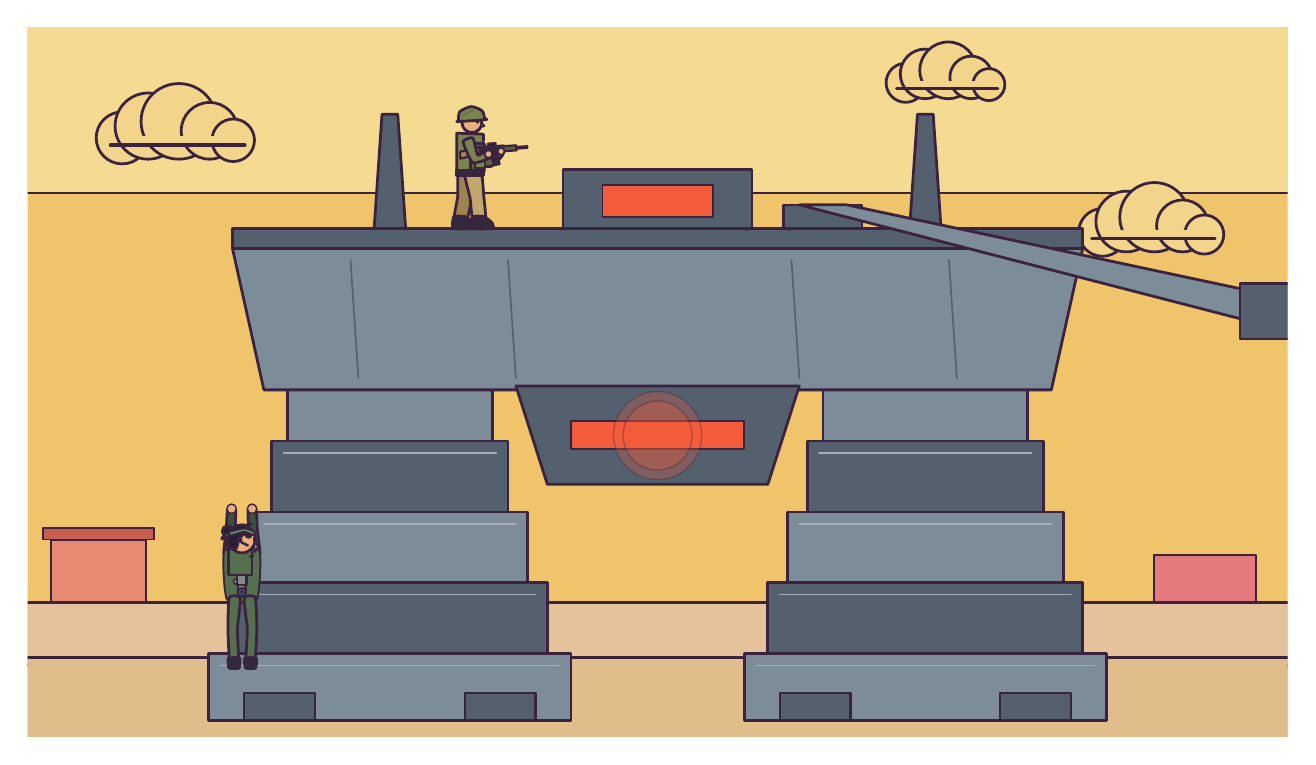
\begin{tikzpicture}
\useasboundingbox (0,0) rectangle (16,9);
\clip (0,0) rectangle (16,9);
\filldraw[draw=ink, line width=1pt, line join=round, fill=sky] (-0.2,-0.2) -- (16.2,-0.2) -- (16.2,9.2) -- (-0.2,9.2) -- cycle;
\filldraw[draw=ink, line width=0.6pt, line join=round, fill=skyhi] (-0.2,6.9) -- (16.2,6.9) -- (16.2,9.2) -- (-0.2,9.2) -- cycle;
\filldraw[draw=ink, line width=1pt, line join=round, fill=cloud] (1.2,7.6) circle (0.33);
\filldraw[draw=ink, line width=1pt, line join=round, fill=cloud] (1.53,7.75) circle (0.42);
\filldraw[draw=ink, line width=1pt, line join=round, fill=cloud] (1.92,7.81) circle (0.48);
\filldraw[draw=ink, line width=1pt, line join=round, fill=cloud] (2.31,7.69) circle (0.36);
\filldraw[draw=ink, line width=1pt, line join=round, fill=cloud] (2.61,7.57) circle (0.27);
\fill[cloud] (1.2,7.51) rectangle (2.61,7.63);
\draw[ink, line width=1.1pt, line cap=round, line join=round] (1.05,7.51) -- (2.76,7.51);
\filldraw[draw=ink, line width=1pt, line join=round, fill=cloud] (13.65,6.4) circle (0.303);
\filldraw[draw=ink, line width=1pt, line join=round, fill=cloud] (13.952,6.538) circle (0.385);
\filldraw[draw=ink, line width=1pt, line join=round, fill=cloud] (14.31,6.593) circle (0.44);
\filldraw[draw=ink, line width=1pt, line join=round, fill=cloud] (14.667,6.482) circle (0.33);
\filldraw[draw=ink, line width=1pt, line join=round, fill=cloud] (14.942,6.373) circle (0.248);
\fill[cloud] (13.65,6.318) rectangle (14.942,6.428);
\draw[ink, line width=1.1pt, line cap=round, line join=round] (13.512,6.318) -- (15.08,6.318);
\filldraw[draw=ink, line width=1pt, line join=round, fill=cloud] (11.15,8.3) circle (0.248);
\filldraw[draw=ink, line width=1pt, line join=round, fill=cloud] (11.397,8.413) circle (0.315);
\filldraw[draw=ink, line width=1pt, line join=round, fill=cloud] (11.69,8.458) circle (0.36);
\filldraw[draw=ink, line width=1pt, line join=round, fill=cloud] (11.982,8.368) circle (0.27);
\filldraw[draw=ink, line width=1pt, line join=round, fill=cloud] (12.207,8.277) circle (0.203);
\fill[cloud] (11.15,8.232) rectangle (12.207,8.323);
\draw[ink, line width=1.1pt, line cap=round, line join=round] (11.037,8.232) -- (12.32,8.232);
\filldraw[draw=ink, line width=0.8pt, line join=round, fill=concrete] (-0.2,0.9) -- (16.2,0.9) -- (16.2,1.7) -- (-0.2,1.7) -- cycle;
\filldraw[draw=ink, line width=0.8pt, line join=round, fill=wallA] (0.3,1.7) -- (1.5,1.7) -- (1.5,2.5) -- (0.3,2.5) -- cycle;
\filldraw[draw=ink, line width=0.7pt, line join=round, fill=shingle] (0.2,2.5) -- (1.6,2.5) -- (1.6,2.65) -- (0.2,2.65) -- cycle;
\filldraw[draw=ink, line width=0.8pt, line join=round, fill=wallC] (14.3,1.7) -- (15.6,1.7) -- (15.6,2.3) -- (14.3,2.3) -- cycle;
\filldraw[draw=ink, line width=0.8pt, line join=round, fill=paving] (-0.2,-0.2) -- (16.2,-0.2) -- (16.2,1) -- (-0.2,1) -- cycle;
\filldraw[draw=ink, line width=1pt, line join=round, fill=mech] (2.3,0.2) -- (6.9,0.2) -- (6.9,1.05) -- (2.3,1.05) -- cycle;
\draw[mechlight, line width=0.6pt, line cap=round, line join=round] (2.45,0.9) -- (6.75,0.9);
\filldraw[draw=ink, line width=1pt, line join=round, fill=mechdark] (2.6,1.05) -- (6.6,1.05) -- (6.6,1.95) -- (2.6,1.95) -- cycle;
\draw[mechlight, line width=0.6pt, line cap=round, line join=round] (2.75,1.8) -- (6.45,1.8);
\filldraw[draw=ink, line width=1pt, line join=round, fill=mech] (2.85,1.95) -- (6.35,1.95) -- (6.35,2.85) -- (2.85,2.85) -- cycle;
\draw[mechlight, line width=0.6pt, line cap=round, line join=round] (3,2.7) -- (6.2,2.7);
\filldraw[draw=ink, line width=1pt, line join=round, fill=mechdark] (3.1,2.85) -- (6.1,2.85) -- (6.1,3.75) -- (3.1,3.75) -- cycle;
\draw[mechlight, line width=0.6pt, line cap=round, line join=round] (3.25,3.6) -- (5.95,3.6);
\filldraw[draw=ink, line width=1pt, line join=round, fill=mech] (3.3,3.75) -- (5.9,3.75) -- (5.9,4.65) -- (3.3,4.65) -- cycle;
\draw[mechlight, line width=0.6pt, line cap=round, line join=round] (3.45,4.5) -- (5.75,4.5);
\filldraw[draw=ink, line width=0.8pt, line join=round, fill=mechdark] (2.75,0.2) -- (3.65,0.2) -- (3.65,0.55) -- (2.75,0.55) -- cycle;
\filldraw[draw=ink, line width=0.8pt, line join=round, fill=mechdark] (5.55,0.2) -- (6.45,0.2) -- (6.45,0.55) -- (5.55,0.55) -- cycle;
\filldraw[draw=ink, line width=1pt, line join=round, fill=mech] (9.1,0.2) -- (13.7,0.2) -- (13.7,1.05) -- (9.1,1.05) -- cycle;
\draw[mechlight, line width=0.6pt, line cap=round, line join=round] (9.25,0.9) -- (13.55,0.9);
\filldraw[draw=ink, line width=1pt, line join=round, fill=mechdark] (9.4,1.05) -- (13.4,1.05) -- (13.4,1.95) -- (9.4,1.95) -- cycle;
\draw[mechlight, line width=0.6pt, line cap=round, line join=round] (9.55,1.8) -- (13.25,1.8);
\filldraw[draw=ink, line width=1pt, line join=round, fill=mech] (9.65,1.95) -- (13.15,1.95) -- (13.15,2.85) -- (9.65,2.85) -- cycle;
\draw[mechlight, line width=0.6pt, line cap=round, line join=round] (9.8,2.7) -- (13,2.7);
\filldraw[draw=ink, line width=1pt, line join=round, fill=mechdark] (9.9,2.85) -- (12.9,2.85) -- (12.9,3.75) -- (9.9,3.75) -- cycle;
\draw[mechlight, line width=0.6pt, line cap=round, line join=round] (10.05,3.6) -- (12.75,3.6);
\filldraw[draw=ink, line width=1pt, line join=round, fill=mech] (10.1,3.75) -- (12.7,3.75) -- (12.7,4.65) -- (10.1,4.65) -- cycle;
\draw[mechlight, line width=0.6pt, line cap=round, line join=round] (10.25,4.5) -- (12.55,4.5);
\filldraw[draw=ink, line width=0.8pt, line join=round, fill=mechdark] (9.55,0.2) -- (10.45,0.2) -- (10.45,0.55) -- (9.55,0.55) -- cycle;
\filldraw[draw=ink, line width=0.8pt, line join=round, fill=mechdark] (12.35,0.2) -- (13.25,0.2) -- (13.25,0.55) -- (12.35,0.55) -- cycle;
\filldraw[draw=ink, line width=1pt, line join=round, fill=mech] (3,4.4) -- (13,4.4) -- (13.4,6.2) -- (2.6,6.2) -- cycle;
\filldraw[draw=ink, line width=1pt, line join=round, fill=mechdark] (2.6,6.2) -- (13.4,6.2) -- (13.4,6.45) -- (2.6,6.45) -- cycle;
\draw[mechdark, line width=0.6pt, line cap=round, line join=round] (4.2,4.55) -- (4.1,6.05);
\draw[mechdark, line width=0.6pt, line cap=round, line join=round] (6.2,4.55) -- (6.1,6.05);
\draw[mechdark, line width=0.6pt, line cap=round, line join=round] (9.8,4.55) -- (9.7,6.05);
\draw[mechdark, line width=0.6pt, line cap=round, line join=round] (11.8,4.55) -- (11.7,6.05);
\filldraw[draw=ink, line width=1pt, line join=round, fill=mechdark] (6.6,3.2) -- (9.4,3.2) -- (9.8,4.45) -- (6.2,4.45) -- cycle;
\filldraw[draw=ink, line width=0.8pt, line join=round, fill=visor] (6.9,3.65) -- (9.1,3.65) -- (9.1,4) -- (6.9,4) -- cycle;
\filldraw[draw=ink, line width=0.5pt, line join=round, fill=visor, fill opacity=0.28, draw opacity=0.35] (8,3.82) circle (0.56);
\filldraw[draw=ink, line width=0.5pt, line join=round, fill=visor, fill opacity=0.28, draw opacity=0.35] (8,3.82) circle (0.438);
\filldraw[draw=ink, line width=1pt, line join=round, fill=mechdark] (6.8,6.45) -- (9.2,6.45) -- (9.2,7.2) -- (6.8,7.2) -- cycle;
\filldraw[draw=ink, line width=0.7pt, line join=round, fill=visor] (7.3,6.6) -- (8.7,6.6) -- (8.7,7) -- (7.3,7) -- cycle;
\filldraw[draw=ink, line width=1pt, line join=round, fill=mechdark] (4.4,6.45) -- (4.8,6.45) -- (4.7,7.9) -- (4.5,7.9) -- cycle;
\filldraw[draw=ink, line width=1pt, line join=round, fill=mechdark] (11.2,6.45) -- (11.6,6.45) -- (11.5,7.9) -- (11.3,7.9) -- cycle;
\filldraw[draw=ink, line width=0.8pt, line join=round, fill=mechdark] (9.6,6.45) -- (10.6,6.45) -- (10.6,6.75) -- (9.6,6.75) -- cycle;
\filldraw[draw=ink, line width=1pt, line join=round, fill=mech] (9.8,6.75) -- (10.4,6.75) -- (15.8,5.6) -- (15.8,5.2) -- cycle;
\filldraw[draw=ink, line width=0.8pt, line join=round, fill=mechdark] (15.4,5.05) -- (16.2,5.05) -- (16.2,5.75) -- (15.4,5.75) -- cycle;
\filldraw[draw=ink, line width=1pt, line join=round, fill=olivedark] plot[smooth cycle, tension=0.3] coordinates {(5.605,7.37) (5.86,7.341) (5.966,7.449) (6.032,7.383) (5.886,7.239) (5.595,7.252)};
\filldraw[draw=ink, line width=1pt, line join=round, fill=khakidark] plot[smooth cycle, tension=0.3] coordinates {(5.684,7.176) (5.637,6.837) (5.573,6.54) (5.417,6.57) (5.462,6.861) (5.474,7.194)};
\filldraw[draw=ink, line width=1pt, line join=round, fill=leather] plot[smooth cycle, tension=0.25] coordinates {(5.403,6.45) (5.671,6.45) (5.655,6.526) (5.558,6.601) (5.411,6.601)};
\filldraw[draw=ink, line width=1pt, line join=round, fill=khaki] plot[smooth cycle, tension=0.3] coordinates {(5.754,7.202) (5.792,6.861) (5.814,6.563) (5.655,6.547) (5.618,6.837) (5.547,7.168)};
\filldraw[draw=ink, line width=1pt, line join=round, fill=leather] plot[smooth cycle, tension=0.25] coordinates {(5.642,6.45) (5.911,6.45) (5.894,6.526) (5.797,6.601) (5.65,6.601)};
\filldraw[draw=ink, line width=1pt, line join=round, fill=olive] (5.449,7.13) -- (5.776,7.13) -- (5.789,7.647) -- (5.449,7.66) -- cycle;
\filldraw[draw=ink, line width=1pt, line join=round, fill=olivedark] (5.621,7.164) -- (5.797,7.172) -- (5.802,7.521) -- (5.634,7.542) -- cycle;
\filldraw[draw=ink, line width=0.7pt, line join=round, fill=olive] (5.676,7.214) -- (5.802,7.214) -- (5.802,7.332) -- (5.676,7.332) -- cycle;
\filldraw[draw=ink, line width=0.7pt, line join=round, fill=olive] (5.676,7.366) -- (5.802,7.366) -- (5.802,7.483) -- (5.676,7.483) -- cycle;
\filldraw[draw=ink, line width=0.8pt, line join=round, fill=leather] (5.44,7.122) -- (5.789,7.122) -- (5.789,7.189) -- (5.44,7.189) -- cycle;
\filldraw[draw=ink, line width=0.7pt, line join=round, fill=skin] (5.592,7.647) -- (5.701,7.647) -- (5.701,7.702) -- (5.592,7.702) -- cycle;
\filldraw[draw=ink, line width=1pt, line join=round, fill=skin] (5.642,7.794) circle (0.126);
\filldraw[draw=ink, line width=0.6pt, line join=round, fill=skin] (5.76,7.794) -- (5.802,7.752) -- (5.755,7.735) -- cycle;
\filldraw[draw=ink, line width=0.3pt, line join=round, fill=ink] (5.713,7.802) circle (0.017);
\draw[ink, line width=0.42pt, line cap=round, line join=round] (5.684,7.844) -- (5.739,7.84);
\draw[ink, line width=0.336pt, line cap=round, line join=round] (5.701,7.71) -- (5.751,7.71);
\filldraw[draw=ink, line width=1pt, line join=round, fill=olive] plot[smooth cycle, tension=0.45] coordinates {(5.47,7.822) (5.488,7.933) (5.634,7.998) (5.772,7.943) (5.803,7.85) (5.814,7.832) (5.467,7.808)};
\draw[olivedark, line width=0.336pt, line cap=round, line join=round] (5.523,7.884) -- (5.661,7.954);
\filldraw[draw=ink, line width=0.8pt, line join=round, fill=wood] (5.496,7.336) -- (5.743,7.401) -- (5.738,7.481) -- (5.49,7.424) -- cycle;
\filldraw[draw=ink, line width=0.8pt, line join=round, fill=leather] (5.744,7.394) -- (6.05,7.415) -- (6.044,7.503) -- (5.738,7.481) -- cycle;
\filldraw[draw=ink, line width=0.8pt, line join=round, fill=leather] (5.879,7.403) -- (5.959,7.409) -- (5.993,7.267) -- (5.922,7.254) -- cycle;
\filldraw[draw=ink, line width=0.8pt, line join=round, fill=olivedark] (6.01,7.428) -- (6.209,7.442) -- (6.204,7.506) -- (6.005,7.492) -- cycle;
\filldraw[draw=ink, line width=0.7pt, line join=round, fill=hairdark] (6.207,7.462) -- (6.346,7.472) -- (6.345,7.496) -- (6.206,7.486) -- cycle;
\filldraw[draw=ink, line width=0.7pt, line join=round, fill=hairdark] (5.845,7.489) -- (5.945,7.496) -- (5.942,7.535) -- (5.843,7.528) -- cycle;
\filldraw[draw=ink, line width=1pt, line join=round, fill=olive] plot[smooth cycle, tension=0.3] coordinates {(5.654,7.599) (5.716,7.379) (5.834,7.442) (5.87,7.348) (5.652,7.285) (5.529,7.552)};
\filldraw[draw=ink, line width=0.7pt, line join=round, fill=skin] (5.852,7.395) circle (0.05);
\filldraw[draw=ink, line width=0.7pt, line join=round, fill=skin] (6.012,7.429) circle (0.046);
\filldraw[draw=ink, line width=1pt, line join=round, fill=camoB] plot[smooth cycle, tension=0.3] coordinates {(2.491,2.315) (2.522,2.614) (2.54,2.882) (2.64,2.878) (2.632,2.606) (2.611,2.305)};
\filldraw[draw=ink, line width=0.5pt, line join=round, fill=skin] (2.59,2.89) circle (0.06);
\filldraw[draw=ink, line width=1pt, line join=round, fill=camoB] plot[smooth cycle, tension=0.3] coordinates {(2.829,2.305) (2.808,2.606) (2.8,2.878) (2.9,2.882) (2.918,2.614) (2.949,2.315)};
\filldraw[draw=ink, line width=0.5pt, line join=round, fill=skin] (2.85,2.89) circle (0.06);
\filldraw[draw=ink, line width=0.7pt, line join=round, fill=suit] plot[smooth cycle, tension=0.3] coordinates {(2.5,2.36) (2.94,2.36) (2.91,1.74) (2.53,1.74)};
\filldraw[draw=ink, line width=0.55pt, line join=round, fill=camoA] plot[smooth cycle, tension=0.5] coordinates {(2.783,2.145) (2.741,2.18) (2.702,2.141) (2.693,2.09) (2.747,2.079) (2.818,2.104)};
\filldraw[draw=ink, line width=0.55pt, line join=round, fill=camoA] plot[smooth cycle, tension=0.5] coordinates {(2.638,1.932) (2.707,1.939) (2.749,1.958) (2.729,1.995) (2.671,2.001) (2.612,1.983)};
\filldraw[draw=ink, line width=0.9pt, line join=round, fill=metal] (2.768,1.845) -- (2.768,2.175) -- (2.672,2.175) -- (2.672,1.845) -- cycle;
\filldraw[draw=ink, line width=0.8pt, line join=round, fill=chromedark] (2.779,1.922) -- (2.779,2.098) -- (2.661,2.098) -- (2.661,1.922) -- cycle;
\filldraw[draw=ink, line width=0.8pt, line join=round, fill=portalblue] (2.72,1.83) circle (0.053);
\filldraw[draw=ink, line width=0.6pt, line join=round, fill=portalbluehi] (2.72,1.83) circle (0.024);
\filldraw[draw=ink, line width=0.8pt, line join=round, fill=portalorange] (2.72,2.19) circle (0.053);
\filldraw[draw=ink, line width=0.6pt, line join=round, fill=portalorangehi] (2.72,2.19) circle (0.024);
\filldraw[draw=ink, line width=1pt, line join=round, fill=suit] plot[smooth cycle, tension=0.3] coordinates {(2.7,1.755) (2.663,1.359) (2.676,0.983) (2.566,0.977) (2.543,1.361) (2.56,1.765)};
\filldraw[draw=ink, line width=0.5pt, line join=round, fill=leather] plot[smooth cycle, tension=0.3] coordinates {(2.541,1) (2.701,1) (2.691,0.86) (2.551,0.86)};
\filldraw[draw=ink, line width=1pt, line join=round, fill=suit] plot[smooth cycle, tension=0.3] coordinates {(2.89,1.765) (2.91,1.361) (2.885,0.977) (2.775,0.983) (2.79,1.359) (2.75,1.755)};
\filldraw[draw=ink, line width=0.5pt, line join=round, fill=leather] plot[smooth cycle, tension=0.3] coordinates {(2.75,1) (2.91,1) (2.9,0.86) (2.76,0.86)};
\filldraw[draw=ink, line width=0.8pt, line join=round, fill=suit] (2.55,2.05) -- (2.85,2.05) -- (2.85,2.45) -- (2.55,2.45) -- cycle;
\filldraw[draw=ink, line width=1pt, line join=round, fill=skin] (2.72,2.5) circle (0.17);
\filldraw[draw=ink, line width=0.7pt, line join=round, fill=skin] (2.876,2.52) -- (2.924,2.4) -- (2.882,2.34) -- cycle;
\filldraw[draw=ink, line width=0.3pt, line join=round, fill=ink] (2.805,2.56) circle (0.045);
\draw[ink, line width=1.2pt, line cap=round, line join=round] (2.774,2.67) -- (2.839,2.7);
\draw[ink, line width=0.9pt, line cap=round, line join=round] (2.825,2.28) -- (2.865,2.3);
\filldraw[draw=ink, line width=1pt, line join=round, fill=hairdark] plot[smooth cycle, tension=0.45] coordinates {(2.547,2.406) (2.542,2.551) (2.618,2.662) (2.754,2.684) (2.865,2.605) (2.814,2.571) (2.729,2.559) (2.678,2.483) (2.644,2.381)};
\filldraw[draw=ink, line width=1pt, line join=round, fill=hairdark] (2.542,2.605) circle (0.071);
\filldraw[draw=ink, line width=0.7pt, line join=round, fill=greenD] plot[smooth cycle, tension=0.3] coordinates {(2.553,2.593) (2.754,2.641) (2.884,2.597) (2.869,2.556) (2.754,2.597) (2.564,2.55)};
\filldraw[draw=ink, line width=0.7pt, line join=round, fill=greenD] plot[smooth cycle, tension=0.3] coordinates {(2.56,2.558) (2.471,2.5) (2.459,2.517) (2.54,2.585)};
\filldraw[draw=ink, line width=0.7pt, line join=round, fill=leather] (2.695,2.491) circle (0.022);
\draw[ink, line width=0.9pt, line cap=round, line join=round] (2.712,2.466) -- (2.796,2.423);
\end{tikzpicture}
\end{document}
